\begin{frame}
  \frametitle{Customize your board device tree!}
  \small
    \begin{itemize}
    \item Kernel developpers write {\em Device Tree Sources (DTS)},
      which become {\em Device Tree Blobs (DTB)} once compiled.
    \item There is one different Device Tree for each board/platform
      supported by the kernel, available in
      \code{arch/<arch>/boot/dts/<board>.dtb}. Their purpose is:
      \begin{columns}
        \column{0.65\textwidth}
        \begin{itemize}
        \item To describe external devices attached to non-discoverable
          busses and configure them.
        \item To configure pin muxing: choosing what SoC signals are
          made available on the board external connectors.
          See \url{http://linux.tanzilli.com/} for a web service doing this
          interactively.
        \item To configure some system parameters: flash partitions,
          kernel command line (other ways exist)
        \end{itemize}
        \column{0.35\textwidth}
        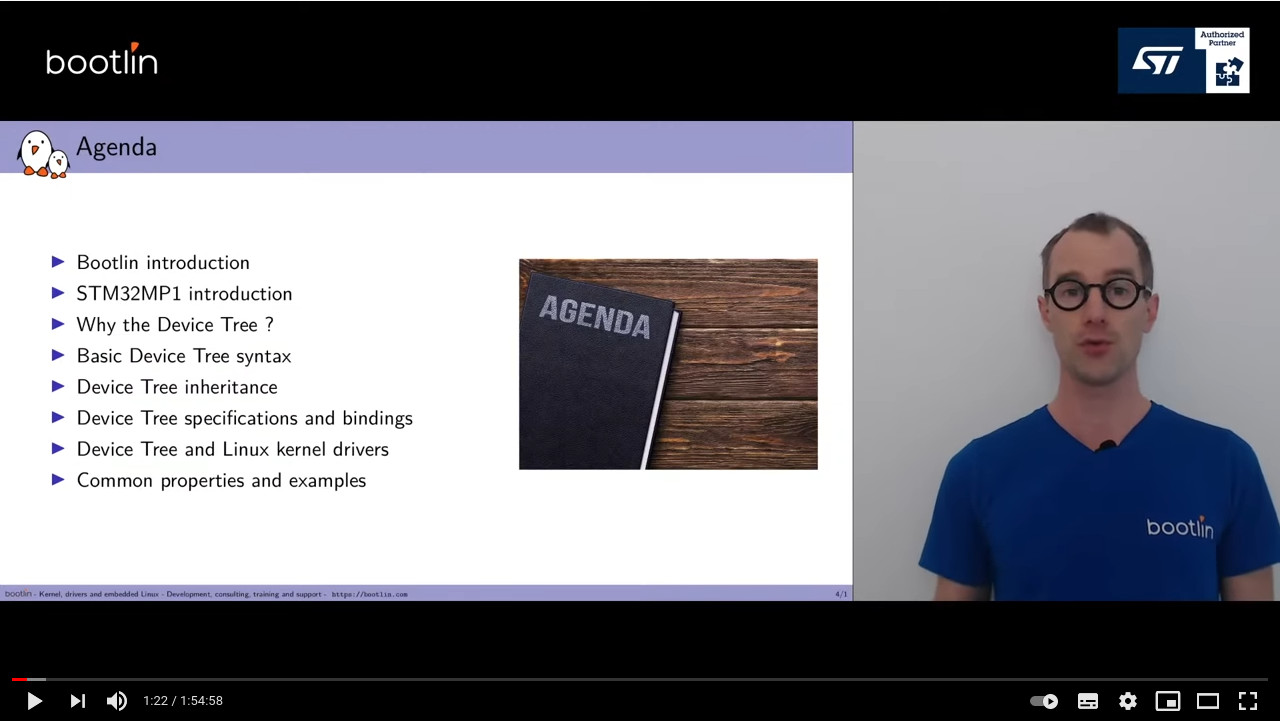
\includegraphics[width=\textwidth]{common/device-tree-video.jpg}
      \end{columns}
    \item Device Tree 101 webinar, Thomas Petazzoni (2021):\\
      Slides: \url{https://bootlin.com/blog/device-tree-101-webinar-slides-and-videos/}\\
      Video: \url{https://youtu.be/a9CZ1Uk3OYQ}
    \end{itemize}
\end{frame}
